\section*{Multiple-choice}\label{sec:mc}

Dine svar skal indtastes i ITX-systemets multiple-choice modul.

\multiplechoicestart

\spoergsmaal{MergeSort og sammenligninger}
Betragt følgende input til {\sc MergeSort}, implementeret som i CLRS sektion 2.3.
\begin{center}
\begin{tabular}{|c|c|c|c|}
\hline
4 & 3 & 1 & 2\\
\hline
\end{tabular}
\end{center}
Hvor mange sammenligninger af to elementer laver {\sc MergeSort} totalt på dette input?
Sammenligninger med $\infty$ i {\sc Merge} skal ikke tælles med.
\etsvar
\mulighederstart
\svar Der laves 3 sammenligninger
\svar Der laves 4 sammenligninger\korrekt
\svar Der laves 5 sammenligninger
\svar Der laves 6 sammenligninger
\svar Der laves 7 sammenligninger
\mulighederslut
\forklaring{
De to rekursive kald på listerne $\langle 4,3\rangle$ og $\langle 1,2\rangle$ bruger hver én sammenligning.
Efter disse kald flettes de sorterede lister $\langle 3,4\rangle$ og $\langle 1,2\rangle$.
Denne fletning bruger to sammenligninger: $3$ mod $1$ og derefter $3$ mod $2$.
Totalt bruges derfor $1+1+2=4$ sammenligninger.
}


\spoergsmaal{Asymptotiske grænser}
Hvilke af nedenstående køretider er $O(n^2)$?
\fleresvar
\mulighederstart
\svar{$2^{\lg n}$}\korrekt
\svar{$n^3$}
\svar{$1.5^n$}
\svar{$\sqrt{n}$}\korrekt
\svar{$\lg n$}\korrekt
\mulighederslut
\forklaring{
Vi undersøger om hver funktion vokser højst kvadratisk.
$2^{\lg n} = n$, da $\lg n = \log_2 n$, og derfor er $2^{\lg n} = n$. Dermed er funktionen også $O(n^2)$.
Derimod vokser $n^3$ hurtigere end $n^2$ og er derfor ikke $O(n^2)$.
$1.5^{n}$ vokser hurtigere end ethvert polynomium i~$n$, herunder $n^2$, og er derfor ikke $O(n^2)$.
Endelig vokser $\sqrt{n} = n^{1/2}$ og $\log n$ begge asymptotisk langsommere end $n^2$, så de er $O(n^2)$.
}


\spoergsmaal{Løsning af rekursionsligninger}
Antag at $n$ er en potens af 2, at $T_i(1)=1$ for $i=1,\dots,6$ og betragt rekursionsligningerne nedenfor. Hvilke af følgende udsagn er sande?
\fleresvar
\mulighederstart
\svar $T_1(n) = 2\,T_1(n/2) + n \log n$ har løsning $T_1(n) = \Theta(n \log n)$.
\svar $T_2(n) = 4\,T_2(n/4) + n^2$ har løsning $T_2(n) = \Theta(n^2)$.\korrekt
\svar $T_3(n) = 4\,T_3(n/2) + n$ har løsning $T_3(n) = \Theta(n^2)$.\korrekt
\svar $T_4(n) = 4\,T_4(n/2) + n^2$ har løsning $T_4(n) = \Theta(n^2)$.
\svar $T_5(n) = 8\,T_5(n/2) + n^2 \log n$ har løsning $T_5(n) = \Theta(n^3)$.\korrekt
\svar $T_6(n) = 8\,T_6(n/2) + n^3$ har løsning $T_6(n) = \Theta(n^3)$.
\mulighederslut
\forklaring{Master theorem kan bruges til at finde en løsning på alle rekursionsligningerne:
Skriv $T(n)=aT(n/b)+f(n)$ og sammenlign $f(n)$ med $n^{\log_b a}$.
\begin{enumerate}
    \item $a=2,b=2$: $n^{\log_b a}=n$, og $f(n)=n\log n=\Theta(n^{\log_b a}\log n)$, så $T_1(n)=\Theta(n\log^2 n)$ (udsagnet er falsk).
\item $a=4,b=4$: $n^{\log_b a}=n$, og $f(n)=n^2=\Omega(n^{1+\varepsilon})$ med regularity $af(n/b)=4(n/4)^2=n^2/4\le c n^2$, så $T_2(n)=\Theta(n^2)$ (sand).
\item $a=4,b=2$: $n^{\log_b a}=n^2$, og $f(n)=n=O(n^{2-\varepsilon})$, så $T_3(n)=\Theta(n^2)$ (sand).
\item $a=4,b=2$: $n^{\log_b a}=n^2$, og $f(n)=n^2=\Theta(n^{\log_b a})$, så $T_4(n)=\Theta(n^2\log n)$ (falsk).
\item $a=8,b=2$: $n^{\log_b a}=n^3$, og $f(n)=n^2 \log n = O(n^{3-\varepsilon})$, så $T_5(n)=\Theta(n^3)$ (sand).
\item $a=8,b=2$: $n^{\log_b a}=n^3$, og $f(n)=n^3=\Theta(n^{\log_b a})$, så $T_6(n)=\Theta(n^3\log n)$ (falsk).
\end{enumerate}
}


\spoergsmaal{Opskrivning af rekursionsligning}
Betragt følgende rekursive algoritme:
\begin{codebox}
  \Procname{$\proc{RecursiveMystery}(A,i,j)$}
  \li \If $i \ge j$
  \li \Then
        \Return $0$
      \End
  \li $q \gets \lfloor (i+j)/2 \rfloor$
  \li $x \gets \proc{RecursiveMystery}(A,i,q)$
  \li $y \gets \proc{RecursiveMystery}(A,q+1,j)$
  \li $c \gets 0$
  \li \For $p \gets i$ \To $q$
  \li \Do
        \For $r \gets q+1$ \To $j$
  \li   \Do
          \If $A[p] = A[r]$
  \li     \Then
            $c \gets c+1$
          \End
        \End
      \End
  \li \Return $x+y+c$
\end{codebox}
Antag at \(n\) er en potens af 2, og at alle elementære operationer tager konstant tid.
Hvilken rekursionsligning beskriver bedst køretiden \(T(n)\) for følgende kald?
\[
\proc{RecursiveMystery}(A,1,n)
\]
\etsvar
\mulighederstart
\svar \(T(n)=T(n/2)+\Theta(n)\)
\svar \(T(n)=T(n/2)+\Theta(n^2)\)
\svar \(T(n)=2T(n/2)+\Theta(n)\)
\svar \(T(n)=2T(n/2)+\Theta(n^2)\) \korrekt
\svar \(T(n)=3T(n/2)+\Theta(n)\)
\svar \(T(n)=3T(n/2)+\Theta(n^2)\)
\mulighederslut

\forklaring{
For \(n>1\) laver algoritmen to rekursive kald, og hvert kald arbejder på en halvdel af arrayet med inputstørrelse \(n/2\).
Det giver bidraget \(2T(n/2)\).
Efter de rekursive kald tæller de to indlejrede løkker antallet af par af ens elementer, hvor det ene element ligger i venstre halvdel og det andet i højre halvdel.
Der er \((n/2)\cdot(n/2)=\Theta(n^2)\) sådanne par, og testen samt en eventuel optælling tager konstant tid for hvert par.
Køretiden beskrives derfor af
\[
T(n)=2T(n/2)+\Theta(n^2),
\]
med basistilfældet \(T(1)=\Theta(1)\).
}



\spoergsmaal{Køretidsanalyse}
Betragt følgende algoritme der som input tager et positivt heltal $n$:

\begin{codebox}
  \Procname{$\proc{TripleLoopMystery}(n)$}
  \li $s \gets 0$
  \li \For $i \gets 1$ \To $n$ \Do
  \li \For $j \gets 1$ \To $i$ \Do
  \li $k \gets 1$
  \li \While $k \le n$ \Do
  \li $s \gets s + 1$
  \li $k \gets 4k$ \End \End \End
  \li \Return $s$
\end{codebox}
Antag at alle elementære operationer tager konstant tid.  
Hvad er algoritmens asymptotiske køretid som funktion af $n$?
\etsvar
\mulighederstart
\svar{$\Theta(n^2)$}
\svar{$\Theta(n^2 \log n)$}\korrekt
\svar{$\Theta(n^3)$}
\svar{$\Theta(n^3 \log n)$}
\svar{$\Theta(n^4)$}
\svar{$\Theta(n^4 \log n)$}
\mulighederslut
\forklaring{
Den yderste \For-løkke kører $n$ gange. Den næste \For-løkke kører $i$ gange, så det totale antal par $(i,j)$ er
$\sum_{i=1}^{n} i = \Theta(n^2)$.
For hvert sådant par firedobles $k$ i \While-løkken, så den kører $\Theta(\log n)$ gange.
Dermed er den samlede køretid $\Theta(n^2 \log n)$.
}



\spoergsmaal{Dynamiske tabeller}
Vi betragter dynamiske tabeller som beskrevet i CLRS sektion 16.4.2
(versionen med både {\sc Table-Insert} og {\sc Table-Delete}).
En tom tabel $T$ initialiseres med
\[
T.num = 0,\qquad T.size = 0.
\]

Derefter udføres følgende operationer i rækkefølge:
{\sc Insert, Insert, Insert, Insert, Insert,
Delete, Delete, Delete, Delete,
Insert, Insert, Insert.}
Hvilke af følgende udsagn er sande efter den sidste operation?
\fleresvar
\mulighederstart
\svar $T.num = 4$ \korrekt
\svar $T.num = 5$
\svar $T.num = 6$
\svar $T.size = 4$ \korrekt
\svar $T.size = 8$
\svar $T.size = 16$
\mulighederslut

\forklaring{
Efter de første fem indsættelser gælder
\[
(T.num,T.size)=(5,8).
\]

Efter tre sletninger er tilstanden $(2,8)$, og belastningsgraden er præcis $1/4$, så tabellen halveres ikke (endnu).
Efter den fjerde sletning bliver den midlertidige tilstand $(1,8)$, hvor belastningsgraden er strengt mindre end $1/4$, og tabellen halveres derfor til størrelse 4:
\[
(5,8)\rightarrow(4,8)\rightarrow(3,8)\rightarrow(2,8)\rightarrow(1,8)\rightarrow(1,4).
\]

De sidste tre indsættelser giver
\[
(1,4)\rightarrow(2,4)\rightarrow(3,4)\rightarrow(4,4).
\]
Ingen af disse udløser en fordobling, så sluttilstanden er
\(
T.num=4, T.size=4
\).
}


\spoergsmaal{Fibonaccihobe}
I Fibonaccihobe (jf. CLRS digitalt kapitel 19) er potentialfunktionen givet ved
\[
\Phi(H)=t(H)+2\,m(H),
\]
hvor \(t(H)\) er antallet af knuder i rodlisten og \(m(H)\) antallet af markerede knuder.
Antag at vi har en Fibonaccihob $H$ med minimumsværdi 10 (dvs. {\sc Minimum}\((H)\) returnerer nøglen med værdi~10).
Lad $x$ være en nøgle i $H$ med værdi $87$.
Hvilke af følgende operationer på \(H\) vil \emph{altid} få potentialfunktionen til at stige (ud fra de angivne egenskaber)?
\fleresvar
\mulighederstart
\svar {\sc Minimum}\((H)\)
\svar {\sc Fib-Heap-Decrease-Key}\((H,x,42)\)
\svar {\sc Fib-Heap-Delete}\((H,x)\)
\svar {\sc Fib-Heap-Insert}\((H,5)\) \korrekt
\svar {\sc Fib-Heap-Insert}\((H,30)\) \korrekt
\mulighederslut
\forklaring{
En {\sc Minimum}-operation ændrer ikke hoben, men returnerer kun en pointer til minimumsknuden. Derfor ændres hverken \(t(H)\) eller \(m(H)\), og potentialet stiger ikke.

En {\sc Fib-Heap-Decrease-Key}-operation får kun potentialet til at stige i nogle tilfælde. Hvis \(x\) for eksempel allerede er en rod, eller hvis den nye nøgle 42 stadig ikke bryder heap-ordenen i forhold til \(x\)'s forælder, sker der ingen cut operation og \(t(H)\) og \(m(H)\) er uændrede.

En {\sc Fib-Heap-Delete}-operation udføres ved først at sænke nøglen til \(-\infty\) med {\sc Fib-Heap-Decrease-Key} og derefter lave {\sc Fib-Heap-Extract-Min}. Decrease-Key-skridtet kan markere en knude (ved et cascading cut), men {\sc Extract-Min} markerer ikke knuder; derimod kan den fjerne rødder under konsolidering af rodlisten (og fjerne markeringer, når knuder linkes). Derfor er der ikke en garanteret stigning i \(\Phi(H)\).

En {\sc Fib-Heap-Insert}-operation indsætter altid den nye knude som en umarkeret rod i rodlisten. Dermed stiger \(t(H)\) med 1, mens \(m(H)\) er uændret, uanset værdien af den nye nøgle.
}



\spoergsmaal{Rød-sorte invarianter}
Hvilke af følgende udsagn gælder altid for rød-sorte søgetræer (er invarianter eller konsekvenser af invarianter)?
\fleresvar
\mulighederstart
\svar{Alle sorte knuder har præcis to børn.}
\svar{Hver knude er enten rød eller sort.}\korrekt
\svar{Træets højde er $\Theta(\log n)$.}\korrekt
\svar{Hvis en knude er rød, så er begge dens børn sorte.}\korrekt
\svar{Alle røde knuder har præcis ét barn.}
\svar{For enhver knude $x$ har alle simple stier fra $x$ til et blad samme antal sorte knuder.}\korrekt
\svar{Roden er sort.}\korrekt
\svar{Alle blade (NIL-sentinels) er sorte.}\korrekt
\mulighederslut
\forklaring{Udsagn 2, 4, 6, 7, 8 er netop de fem klassiske rød-sorte egenskaber: knuder er farvet rød/sort, roden er sort, NIL-blade er sorte, røde knuder har sorte børn, og alle veje fra en knude til et blad har samme antal sorte knuder (samme black-height). Udsagn 3 om højden er en konsekvens af de klassiske invarianter, og derfor også selv en gyldig invariant. De to strukturelle udsagn om antal børn gælder ikke generelt.}


\spoergsmaal{Gør algoritmen færdig}
Betragt følgende algoritme (med en uspecificeret del) der er en variant af \proc{Greedy-Activity-Selector} i CLRS sektion 15.1.
Algoritmen skal tage hensyn til en ledelsesbeslutning om, at der ikke må lægges aktiviteter der overlapper med frokostpausen kl. 12--13.
Som input tager algoritmen to arrays $s[1{:}n]$, $f[1{:}n]$ med heltal i $\{0,1,\dots,23\}$, og deres længde~$n$.
Her er $s[i]$ og $f[i]$ henholdsvis start- og sluttidpunkt for aktivitet $a_i$ (hvor $s[i]<f[i]$).
Vi antager at aktiviteterne er sorterede således at sluttidspunkterne i $f$ ligger i ikke-aftagende rækkefølge, at ingen aktiviteter går hen over midnat, og at $a_1$ ikke overlapper med frokostpausen.
\begin{codebox}
\Procname{$\proc{Greedy-Activity-Selector-With-Lunch-Break}(s,f,n)$}
\li $A = \{a_1\}$
\li $k = 1$
\li \For $m = 2$ \To $n$
\li \Do
      \If $s[m] \ge f[k]$ {\bf and} $<${\sc Indsæt kode her}$>$
\li   \Then
        $A = A \cup \{a_m\}$
\li     $k = m$
      \End
    \End
\li \Return $A$
\end{codebox}
Hvilket udtryk skal erstatte $<${\sc Indsæt kode her}$>$ for at få en algoritme der skemalægger et maksimalt antal aktiviteter med denne begrænsning?
\etsvar
\mulighederstart
\svar{ ($s[m] < 13$ {\bf and} $f[k] > 12$) }
\svar{ ($s[m] < 13$ {\bf and} $f[m] > 12$) }
\svar{ ($s[m]\ge 13$ {\bf or} $f[k]\leq 12$) }
\svar{ ($s[m]\ge 13$ {\bf or} $f[m]\leq 12$) }\korrekt
\mulighederslut
\forklaring{Inden $a_m$ inkluderes skal det checkes at intervallet $[s[m],f[m]]$ ikke overlapper med $[12,13]$. Det gælder netop hvis starttidspunktet er tidligst kl. 13 \emph{eller} sluttidspunktet er senest kl. 12.}


\spoergsmaal{Mindste udspændende træ}
Betragt mindste udspændende træ (eng.~\emph{minimum spanning tree}) problemet på denne graf, hvor hver vægt er unik:
\begin{center}
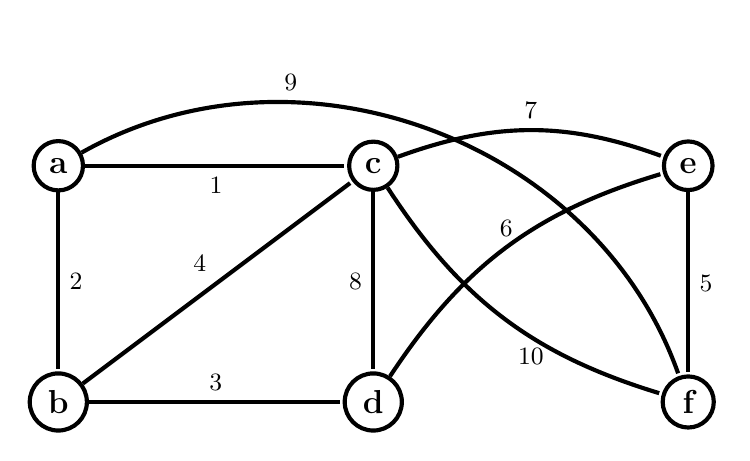
\begin{tikzpicture}[-,>=stealth,shorten >=1pt,auto,
  main node/.style={circle,draw,font=\large\bfseries}, line width=1.5pt]
\node[main node] (a) at (1,1.5) {a};
\node[main node] (b) at (1,-1.5) {b};
\node[main node] (c) at (5,1.5) {c};
\node[main node] (d) at (5,-1.5) {d};
\node[main node] (e) at (9,1.5) {e};
\node[main node] (f) at (9,-1.5) {f};

\path[every node/.style={font=\small}]
(a) edge node {2} (b)
(a) edge[below] node {1} (c)
(a) edge[bend left=50] node[pos=.3, above] {9} (f)
(b) edge node {3} (d)
(b) edge node {4} (c)
(c) edge[left] node {8} (d)
(c) edge[above,bend left=20] node {7} (e)
(d) edge[above,bend left=20] node {6} (e)
(e) edge node {5} (f)
(c) edge[below, bend right=20] node[pos=.6] {10} (f);
\end{tikzpicture}
\end{center}

Hvilke kanter er med i det mindste udspændende træ?
\fleresvar
\mulighederstart
\svar \{a,b\} \korrekt
\svar \{a,c\} \korrekt
\svar \{a,f\}
\svar \{b,c\}
\svar \{b,d\} \korrekt
\svar \{c,d\}
\svar \{c,e\}
\svar \{c,f\}
\svar \{d,e\} \korrekt
\svar \{e,f\} \korrekt
\mulighederslut

\forklaring{
Kør Kruskal: sortér kanter efter vægt og tilføj dem, hvis de ikke danner en kreds.
Først tilføjes \{a,c\} (1), \{a,b\} (2), \{b,d\} (3). Kanten \{b,c\} (4) springes over, da den ville skabe kredsen a--b--c--a.
Derefter tilføjes \{e,f\} (5) og \{d,e\} (6), som forbinder de to komponenter og giver et udspændende træ.
}



\spoergsmaal{Korteste veje}
Betragt følgende vægtede, orienterede graf:
\begin{center}
  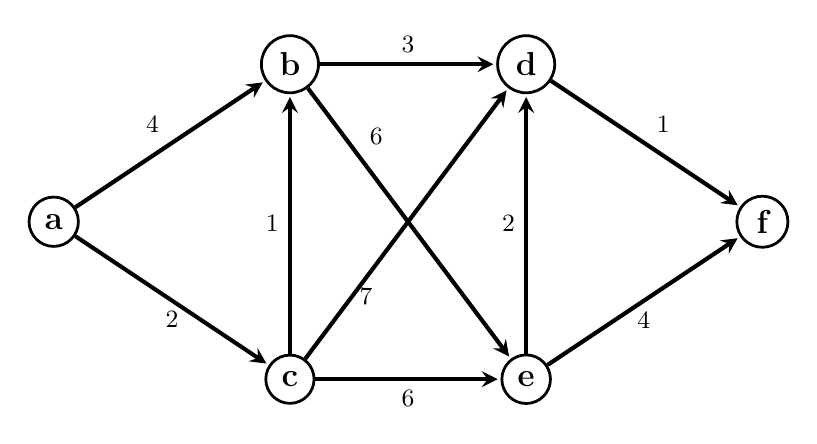
\begin{tikzpicture}[->,>=stealth,shorten >=1pt,auto,
      main node/.style={circle,draw,font=\large\bfseries,line width=1pt}, line width=1.5pt]
  \node[main node] (a) at (0,0) {a};
  \node[main node] (b) at (3,2) {b};
  \node[main node] (c) at (3,-2) {c};
  \node[main node] (d) at (6,2) {d};
  \node[main node] (e) at (6,-2) {e};
  \node[main node] (f) at (9,0) {f};
  \path[every node/.style={font=\small}]
  (a) edge node {4} (b)
  (a) edge[below] node {2} (c)
  (c) edge node {1} (b)
  (c) edge[below] node {6} (e)
  (c) edge node[pos=.3,below] {7} (d)
  (b) edge node {3} (d)
  (b) edge node[pos=.25] {6} (e)
  (e) edge node {2} (d)
  (d) edge node {1} (f)
  (e) edge[below] node {4} (f);
  \end{tikzpicture}
\end{center}

Antag at Dijkstra's algoritme køres med startknude {\bf a}.
I hvilken rækkefølge tages knuderne ud af prioritetskøen?
\etsvar
\mulighederstart
\svar a, c, b, d, e, f
\svar a, c, b, d, f, e \korrekt
\svar a, c, b, e, f, d
\svar a, c, b, e, d, f
\svar a, c, b, f, d, e
\svar a, c, b, f, e, d
\mulighederslut

\forklaring{
Fra startknuden {\bf a} fås først afstandene $d[b]=4$ og $d[c]=2$.
Derfor tages {\bf c} ud som den næste knude.
Kanten $({\bf c},{\bf b})$ forbedrer afstanden til {\bf b} til $3$, så {\bf b} tages ud før de øvrige knuder.
Herefter forbedrer kanten $({\bf b},{\bf d})$ afstanden til {\bf d} til $6$, mens {\bf e} har afstand $8$ via {\bf c}.
Derfor tages {\bf d} ud før {\bf e}.
Kanten $({\bf d},{\bf f})$ giver $d[f]=7$, så {\bf f} tages ud før {\bf e}.
Rækkefølgen bliver derfor a, c, b, d, f, e.
}



\spoergsmaal{Activity selection}
Betragt {\sc Greedy-Activity-Selector} fra CLRS sektion 15.1. Hvilket resultat returnerer algoritmen på følgende input, hvor aktiviteterne allerede er sorteret efter sluttidspunkt:
s = $\langle 1,3,0,5,8,5\rangle$ og f = $\langle 2,4,6,7,9,9\rangle$?
\etsvar
\mulighederstart
\svar A = $\langle a_1,a_2,a_4,a_5\rangle$ \korrekt
\svar A = $\langle a_1,a_2,a_5,a_6\rangle$
\svar A = $\langle a_1,a_3,a_4,a_5\rangle$
\svar A = $\langle a_1,a_3,a_5,a_6\rangle$
\mulighederslut
\forklaring{Håndkørsel af algoritmen giver det viste svar. De andre mulige svar overholder desuden ikke betingelsen at aktiviteterne skal være disjunkte.
}




\spoergsmaal{Længste fælles delsekvens}
Strengene {\tt BANANA} og {\tt ANAGRAM} har begge delsekvensen {\tt ANAA}, og det er en maksimal delsekvens.
Hvor mange forskellige fælles delsekvenser af længde 4 findes der?
\etsvar
\mulighederstart
\svar 1 \korrekt
\svar 2
\svar 3
\svar 4
\mulighederslut
\forklaring{Tegnene G, R og M findes kun i den ene streng og er derfor aldrig med i en fælles delsekvens. Vi kan derfor nøjes med at se på fælles delsekvenser mellem {\tt BANANA} og {\tt ANAA}, og det er tydeligt at kun én har længde 4.

Alternativt (mere generelt): I algoritmen for LCS laves der et vilkårligt valg når cellerne til venstre og over i dynamisk programmerings-tabellen indeholder samme værdi. Det er markeret for vores input i nedenstående tabel:
\begin{center}
\begin{tabular}{c|c|c|c|c|c|c|c|c||}
    &   & A & N & A & G & R & A & M\\
    \hline
     & 0 & 0 & 0 & 0 & 0 & 0 & 0 & 0\\
     \hline
    B & 0 & $\uparrow0$ & $\uparrow0$ & $\uparrow0$ & $\uparrow0$ & $\uparrow0$ & $\uparrow0$ & $\uparrow0$ \\
    A & 0 & $\nwarrow1$ & $\leftarrow1$ & $\nwarrow1$ & $\leftarrow1$ & $\leftarrow1$ & $\nwarrow1$ & $\leftarrow1$ \\
    N & 0 & $\uparrow1$ & $\nwarrow2$ & $\leftarrow2$ & $\leftarrow2$ & $\leftarrow2$ & $\leftarrow2$ & $\leftarrow2$ \\
    A & 0 & $\nwarrow1$ & $\uparrow2$ & $\nwarrow3$ & $\leftarrow3$ & $\leftarrow3$ & $\nwarrow3$ & $\leftarrow3$ \\
    N & 0 & $\uparrow1$ & $\nwarrow2$ & $\uparrow3$ & $\color{red}\uparrow3$ & $\color{red}\uparrow3$ & $\uparrow3$ & $\uparrow3$ \\
    A & 0 & $\nwarrow1$ & $\uparrow2$ & $\nwarrow3$ & $\uparrow3$ & $\uparrow3$ & $\nwarrow4$ & $\leftarrow4$ \\
    \hline
\end{tabular}
\end{center}
\noindent
Vi kan se at selv hvis vi i et eller flere af disse skridt havde valgt $\leftarrow$ i stedet for $\uparrow$ (hvor værdien er 3), ville output stadig være {\tt ANAA}. Derfor er {\tt ANAA} den eneste længste fælles delsekvens.
}




\spoergsmaal{Parallelle algoritmer}
Antag at en parallel algoritme på input af størrelse $n$ har arbejde (eng.~\emph{work}) $T_1=\Theta(n^2)$ og spand (eng.~\emph{span}) $T_\infty=\Theta(n)$.
Vi er interesserede i tiden $T_P$ der bruges til at køre algoritmen på $P$ processorer med grådig opgaveplanlægning (eng.~\emph{greedy scheduling}).
Hvilke af nedenstående påstande er korrekte?
\fleresvar
\mulighederstart
\svar Hvis $P=\Theta(1)$ så er $T_P=O(n^2)$ \korrekt
\svar Hvis $P=\Theta(\log n)$ så er $T_P=O(n \log n)$
\svar Hvis $P=\Theta(n)$ så er $T_P=O(n)$ \korrekt
\svar Hvis $P=\Theta(n^2/\log n)$ så er $T_P=O(\log n)$
\svar Hvis $P=\Theta(n^2)$ så er $T_P=O(1)$
\mulighederslut
\forklaring{Ifølge CLRS Theorem 26.1 er $T_P \leq T_1 / P + T_\infty$, og denne grænse er ifølge Theorem 26.2 indenfor en faktor 2 af den sande køretid. 
Indsættes de givne værdier for $P$ fås:
\begin{align*}
P=\Theta(1) &: \quad T_P=\Theta(n^2+n)=\Theta(n^2) \text{ som er } O(n^2),\\[4pt]
P=\Theta(\log n) &: \quad 
T_P=\Theta\left(\frac{n^2}{\log n}+n\right)
=\Theta\!\left(\frac{n^2}{\log n}\right)\text{ som ikke er } O(n\log n),\\[4pt]
P=\Theta(n) &: \quad T_P=\Theta(n+n)=\Theta(n) \text{ som er } O(n),\\[4pt]
P=\Theta(n^2/\log n) &: \quad 
T_P=\Theta(\log n+n)=\Theta(n) \text{ som ikke er } O(\log n),\\[4pt]
P=\Theta(n^2) &: \quad 
T_P=\Theta(1+n)=\Theta(n) \text{ som ikke er } O(1).
\end{align*}
}



% Let $G = (V,E)$ be a connected simple graph with $|V|=n$ and let $w : E \to \mathbb{N}$ be an edge-weight function. Assume that all weights are distinct (that is, $w$ is an injection). Denote by $M$ the number of minimum spanning trees in $G$ with respect to $w$. Which of the following is always true? 

\spoergsmaal{Mindste udspændende træer}
Lad $G = (V,E)$ være en sammenhængende, simpel graf med $|V|=n$, og lad $w : E \to \mathbb{R}$ være en kantvægtfunktion.
Antag at alle vægte er forskellige (dvs.~at $w$ er injektiv).
Betegn med $M$ antallet af forskellige mindste udspændende træer (eng.~\emph{minimum spanning trees}) i $G$ med hensyn til $w$.
Hvilke af følgende udsagn er altid sande, uanset valg af $G$ og $w$?
\fleresvar
Bemærk at nogle af udsagnene hænger sammen i den forstand at hvis det ene altid gælder så gælder det andet også altid.
\mulighederstart
\svar $M \geq 1$ \korrekt
\svar $M \leq 1$ \korrekt
\svar $M \geq n$
\svar $M \leq n$ \korrekt
\svar Ingen af ovenstående udsagn er altid sande.
\mulighederslut
\forklaring{
% The answer is $M=1$.
% If two different MSTs exist, replace the smallest-weight edge that appears in one but not the other. 
Der er altid præcis ét mindste udspændende træ når alle vægte er forskellige.
Hvis der fandtes to forskellige mindste udspændende træer, kunne man betragte den kant med mindst vægt der optræder i det ene træ, men ikke i det andet, og bruge snit-egenskaben til at udlede en modstrid. Derfor er alle uligheder sande bortset fra $M \geq n$.
}



%Let $T$ be a tree with $n>4$ vertices that is a tree-path going to the right. 
%Here is an illustration with 9 vertices.

\spoergsmaal{Balancering af søgetræer}
For et ulige heltal $n$, lad $T$ være et stærkt ubalanceret binært søgetræ med $n$ nøgler og $(n+1)/2$ knuder på en sti der går mod højre.
Nedenfor er en illustration med $n=9$ nøgler og en sti af længde~5.

\begin{center}
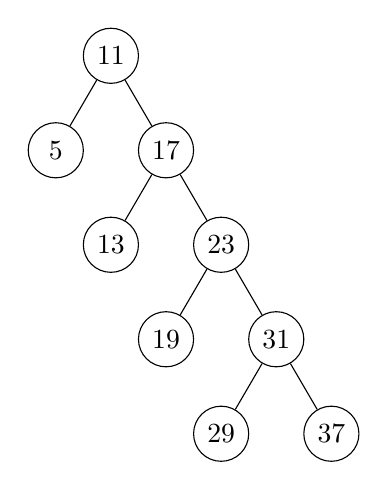
\begin{tikzpicture}[
  every node/.style={
    circle,
    draw,
    minimum size=7mm,
    inner sep=1pt
  },
  edge from parent/.style={draw},
  level distance=12mm,
  sibling distance=14mm
]

\node {11}
  child { node {5} }
  child { node {17}
    child { node {13} }
    child { node {23}
      child { node {19} }
      child { node {31}
        child { node {29} }
        child { node {37} }
      }
    }
  };
\end{tikzpicture}    
\end{center}
%Using asymptotic notation, what is the minimum number of rotations needed to change the tree to have depth at most $10 \log_2(n)$? 
Hvad er det mindste antal rotationer, der skal udføres for at ændre $T$ til at have dybde højst $10 \log_2(n)$?
Vi er interesserede i svaret for store værdier af $n$, udtrykt ved brug af asymptotisk notation.
\etsvar
\mulighederstart
\svar $\Theta(n)$ \korrekt
\svar $\Theta(n \log n)$
\svar $\Theta(n^2)$
\svar $\Theta(n^2 \log n)$
\mulighederslut
\forklaring{
% The answer is $\Theta(n)$. For the upper bound, which is the relevant part for the question, perform the balancing in iterations. In each iteration, left-rotate every second node. After $k$ iterations, every subtree hanging off the current ``right spine'' has height at most $k$.
% And the length of the ``right spine'' becomes $O(n/2^k)$.
Dybden kan højst reduceres med 1 hver gang der laves en rotation, så derfor kræves mindst $\Omega(n)$ rotationer.
Vi argumenterer for at $O(n)$ rotationer er nok:
Rotationerne kan udføres i iterationer, hvor hver iteration udfører en venstrerotation i hver anden knude på stien der går til højre, fx 17 og 31 i eksemplet.
Det reducerer stiens længde med en faktor 2.
Efter $k$ iterationer har hvert undertræ der hænger mod venstre fra den højre sti højde højst $k$.
Derfor bliver dybden af træet højst $O(n/2^k + k)$.
Efter $k=\log_2(n)$ iterationer er dybden af træet højst $2\log_2(n)$.
Antal rotationer i iteration $k$ er $\Theta(n/2^k)$, så totalt er antal rotationer $\Theta(\sum_{k=1}^{\lg n} n/2^k)$ hvilket er $\Theta(n)$.
}

\spoergsmaal{Graham's Scan}
Betragt følgende punktmængde.

\begin{center}
\begin{tikzpicture}[scale=0.75]
  \draw[->] (-0.3,0) -- (5.8,0) node[right] {$x$};
  \draw[->] (0,-0.3) -- (0,5.8) node[above] {$y$};

  \foreach \x/\y/\name in {
    0/0/p_0,
    4/0/p_1,
    2/1/p_2,
    5/3/p_3,
    2/2/p_4,
    3/5/p_5,
    1/4/p_6
  }{
    \fill (\x,\y) circle (2pt);
    \node[above right] at (\x,\y) {$\name$};
  }
\end{tikzpicture}
\end{center}

Antag at \proc{Graham-Scan} (CLRS digitalt kapitel 33) udføres på punktmængden. Punkterne er nummereret som i algoritmen, så $p_0$ er længst til venstre blandt dem med minimum $y$-koordinat, og de øvrige er sorteret efter vinkel
omkring $p_0$ i rækkefølgen
\[
p_1,p_2,p_3,p_4,p_5,p_6.
\]
Stakken $S$ skrives fra bund til top.
Hvilke af følgende er identisk med indholdet af stakken $S$ på et tidspunkt mens algoritmen kører?
(Bemærk at der \emph{ikke} spørges om hvilke punkter, der på et tidspunkt findes på stakken.)
\fleresvar

\mulighederstart
\svar{$\langle p_0,p_1,p_2,p_3,p_4,p_5\rangle$}
\svar{$\langle p_0,p_1,p_3,p_4,p_5\rangle$}
\svar{$\langle p_0,p_1,p_3,p_5\rangle$}\korrekt
\svar{$\langle p_0,p_2,p_3,p_5\rangle$}
\svar{$\langle p_0,p_2,p_1\rangle$}
\svar{$\langle p_0,p_2,p_5,p_6\rangle$}
\mulighederslut

\forklaring{
Efter initialiseringen i linje 6--8 er stakken
\(
\langle p_0,p_1,p_2\rangle
\).
Når $p_3$ behandles, danner $p_1,p_2,p_3$ et ikke-venstresving, så
$p_2$ fjernes. Derefter indsættes $p_3$, og stakken er
\(
\langle p_0,p_1,p_3\rangle
\).
Når $p_4$ behandles, indsættes det uden at der fjernes punkter:
\(
\langle p_0,p_1,p_3,p_4\rangle
\).
Når $p_5$ behandles, danner $p_3,p_4,p_5$ et ikke-venstresving, så
$p_4$ fjernes. Derefter indsættes $p_5$, og stakken er derfor
\(
\langle p_0,p_1,p_3,p_5\rangle
\).
De øvrige svar forekommer ikke. % af forskellige årsager 
}


% Let $G$ be the bipartite graph with two sides $L = \{\ell_1,\ldots,\ell_{10}\}$ and $R = \{r_1,\ldots,r_{10}\}$.
% The edges of $G$ are defined as follows: there is an edge between $\ell_i$ and $r_j$ if and only if $i \leq j$.
% Denote by $N$ the number of perfect matchings in $G$.
% Which of the following is true? 

\spoergsmaal{Perfect matching}
Lad $G$ være en todelt graf med knudemængderne $L = \{\ell_1,\ldots,\ell_{10}\}$ og $R = \{r_1,\ldots,r_{10}\}$ hvor
der er en kant mellem $\ell_i$ og $r_j$ hvis og kun hvis $i \leq j$.
Betegn med $N$ antallet af perfekte parringer (eng.~\emph{perfect matchings}) i $G$.
Hvilket af følgende udsagn er sandt?
\etsvar
\mulighederstart
\svar $N=0$
\svar $N=1$ \korrekt
\svar $N=2$
\svar $N=10$
\svar $N = {10 \choose 2}$
\mulighederslut
\forklaring{
% There is a single perfect matching. Every permutation $\pi$ that is not the identity maps some $i$ to $\pi(i) < i$ so it is not in the graph. The identity matching is present.
Enhver permutation $\pi: \{1,\dots,10\} \to \{1,\dots,10\}$ som ikke er identitetsfunktionen, har et input $i$ med $\pi(i)<i$, så den tilsvarende matching findes ikke i grafen.
Så den eneste matching er den der svarer til identitetsfunktionen.
}


\multiplechoiceslut

\newpage

\section*{Skriftlige opgaver}\label{sec:written}

{\bf Skriftlige opgaver} afleveres som et Word dokument i ITX systemet.
Der er mulighed for at tegne og skrive på tablet, og indsætte i dokumentet.
\begin{itemize}
    \item Brug \emph{én side til hvert delspørgsmål, i samme rækkefølge som i opgavesættet.} 
    \item Delspørgsmålets nummer/bogstav (fx 19 eller 20.a) skal fremgå.
\end{itemize}



\section{Indsættelse i rød-sort søgetræ (4\%)}
Vi starter med et tomt rød-sort binært søgetræ.
Indsæt nøglerne
\[
30,15,45,10
\]
i den angivne rækkefølge ved brug af CLRS' algoritme {\sc RB-Insert}.

\punkt{}{Tegn det resulterende rød-sorte søgetræ, med angivelse af farve på hver knude.}

\forklaring{
Efter indsættelse af 30 bliver knuden roden og farves sort.
Nøglerne 15 og 45 indsættes som røde børn af 30.
Nøglen 10 indsættes som rødt venstre barn til 15.
Da både 15 og dens søskende 45 er røde, omfarves 15 og 45 til sorte, og 30 omfarves midlertidigt til rød, hvorefter roden igen farves sort.
Det resulterende træ er:
\begin{center}
\begin{tikzpicture}[-,>=stealth,level/.style={sibling distance = 4cm/#1,
    level distance = 1cm}, line width=1.5pt] 
  \node [black] {30}
      child{ node [black] {15} 
              child{ node [red] {10} }
              child[missing]
      }
      child{ node [black] {45} };
\end{tikzpicture}
\end{center}
}


\section{Intervaldækning (12\%)}

Vi er givet et tal $L>0$ og en samling af $n$ intervaller
\[
I_i=[a_i,b_i],
\]
hvor $i\in\{1,2,\ldots,n\}$ og $a_i < b_i$.
Vi ønsker at vælge så få intervaller som muligt, således at deres forening dækker hele intervallet $[0,L]$.
Dvs.~at finde $J\subseteq\{1,2,\ldots,n\}$ således at $[0,L]\subseteq\bigcup_{i\in J} I_i$ og $\vert J\vert$ er mindst mulig.
Algoritmen skal returnere størrelsen $\vert J\vert$.

\punkt{a)}
{Lad $L=12$, og lad intervallerne være
\[
[2,8],\ [-1,4],\ [1,5],\ [8,12],\ [6,20],\ [7,9].
\]
Angiv en optimal løsning og argumentér kort for dit svar.}

\forklaring{
En optimal løsning er f.eks.
\[
[-1,4],\ [2,8],\ [6,20].
\]
(Et andet gyldigt valg er $[-1,4]$, $[2,8]$, $[8,12]$).
Disse tre intervaller dækker hele $[0,12]$.
Der findes ingen løsning med kun to intervaller: For at dække $0$ skal vi bruge $[-1,4]$, og intet enkelt interval dækker hele vejen fra $4$ til $12$.
Derfor er tre intervaller optimalt.
}


\punkt{b)}
{Beskriv en effektiv algoritme som finder et minimum antal intervaller der dækker $[0,L]$, hvis en sådan dækning findes.
Hvis $[0,L]$ ikke kan dækkes, skal algoritmen returnere \const{false}.
Input til algoritmen er $(a,b,n,L)$, hvor $a[1{:}n]$ og $b[1{:}n]$ er arrays af længde $n$ med start- og slutpunkter, dvs.~$I_i=[a[i],b[i]]$.
Du må gerne skrive pseudokode, men det er også tilstrækkeligt med en klar og præcis beskrivelse i tekst.
Du skal redegøre for algoritmens køretid -- for at få fuldt point skal den være $O(n\log n)$.}

\forklaring{
Sortér først intervallerne efter venstre endepunkt.
Vi vedligeholder en variabel $x$, som angiver at vi allerede har dækket $[0,x]$.
Til at starte med er $x=0$.
Så længe $x<L$, gennemløber vi alle intervaller der starter senest i $x$, og finder blandt disse det interval der når længst mod højre.
Hvis intet sådant interval når længere end $x$, kan $[0,L]$ ikke dækkes.
Ellers vælger vi intervallet og opdaterer $x$.
For at gennemløbe intervallerne effektivt vedligeholder vi et index $i$, så vi kan starte søgningen fra det senest tilføjede interval.

\begin{codebox}
\Procname{$\proc{CoverInterval}(a,b,n,L)$}
\li sortér intervallerne efter stigende $a[i]$
\li $x \gets 0$
\li $i \gets 1$
\li $k \gets 0$
\li \While $x < L$
\Do
\li     $best \gets x$
\li     \While $i \le n$ \textbf{and} $a[i] \le x$
\Do
\li         \If $b[i] > best$
\li         \Then $best \gets b[i]$
            \End
\li         $i \gets i+1$
        \End
\li     \If $best == x$
\li     \Then \Return \const{false}
        \End
\li     $x \gets best$
\li     $k \gets k+1$
    \End
\li \Return $k$
\end{codebox}

Sorteringen tager $O(n\log n)$ tid.
Efter sorteringen behandles hvert interval højst én gang i det indre while-loop, så resten af algoritmen tager $O(n)$ tid.
Den samlede køretid er derfor $O(n\log n)$.
}

\punkt{c)}
{Argumentér for at algoritmen altid finder et minimum antal intervaller, hvis en dækning findes.}

\forklaring{
Vi viser at det grådige valg er sikkert.
Antag at algoritmen på et tidspunkt har dækket intervallet $[0,x]$.
Enhver gyldig løsning på resten af problemet må benytte et interval $I_i$ der starter senest i $x$, da der ellers ville opstå et hul i dækningen.
Algoritmen vælger blandt alle sådanne intervaller et interval $I_{i^*}$ der når længst muligt mod højre.
Hvis $I_i$ og $I_{i^*}$ er forskellige intervaller, kunne vi erstatte $I_i$ med $I_{i^*}$ og stadig have en gyldig løsning, idet $b[i^*]\geq b[i]$.

Ved induktion i antal intervaller følger det at algoritmens valg kan indgå i en optimal løsning i hvert skridt.
Algoritmen finder derfor det mindst mulige antal intervaller.
}


\section{Opadgående polygonal kæde (12\%)}\label{sec:last}

Vi er givet $n$ punkter i planen
\(
p_i=(x_i,y_i),
\)
hvor $i\in\{1,2,\ldots,n\}$.
Vi antager at alle $x_i$-koordinater er forskellige.
%
En opadgående polygonal kæde er en følge af punkter
\[
p_{i_1},p_{i_2},\ldots,p_{i_k}
\]
hvor der gælder
\[
x_{i_1}<x_{i_2}<\cdots <x_{i_k}
\text{ og }
y_{i_1}<y_{i_2}<\cdots <y_{i_k} \enspace .
\]
Betragt problemet at finde længden $k$ af en længst mulig opadgående polygonal kæde.
Nedenfor ses et eksempel på en punktmængde og en opadgående kæde af længde 3 illustreret som en sti (ikke nødvendigvis den længste).

\begin{center}
\begin{tikzpicture}[scale=0.75]
  \draw[->] (0,0) -- (9,0) node[right] {$x$};
  \draw[->] (0,0) -- (0,7) node[above] {$y$};

  \foreach \x/\y/\name in {
    1/2/$p_1$,
    2/5/$p_2$,
    3/3/$p_3$,
    4/6/$p_4$,
    5/4/$p_5$,
    6/5/$p_6$,
    7/2/$p_7$,
    8/6/$p_8$
  } {
    \fill (\x,\y) circle (2pt);
    \node[above right] at (\x,\y) {\name};
  }

  \draw[thick] (1,2) -- (2,5) -- (4,6);
\end{tikzpicture}
\end{center}

\punkt{a)}
{Betragt punkterne vist i figuren ovenfor, dvs.
\[
\begin{array}{c|cccccccc}
i    & 1&2&3&4&5&6&7&8\\ \hline
x_i  & 1&2&3&4&5&6&7&8\\
y_i  & 2&5&3&6&4&5&2&6
\end{array}
\]
Angiv en længst mulig opadgående polygonal kæde.}

\forklaring{
En længst mulig opadgående polygonal kæde er
\[
p_1,p_3,p_5,p_6,p_8.
\]
Den har længde $5$ og er opadgående, da
\(
2<3<4<5<6
\)
for $y$-koordinaterne, og punkterne allerede står i stigende orden efter $x$-koordinater.
}

\punkt{b)}
{Beskriv en effektiv algoritme der finder længden af en længst mulig opadgående polygonal kæde.
Input til algoritmen er arrays $x[1{:}n]$ og $y[1{:}n]$ af længde $n$, hvor punkt $i$ er $(x[i],y[i])$.
Du skal redegøre for algoritmens køretid -- for at få fuldt point skal den være $O(n^2)$.}

\forklaring{
Sortér først punkterne efter stigende $x$-koordinat.
Lad $D[i]$ være længden af en længst mulig opadgående kæde der slutter i punkt $i$.
Så er
\[
D[i] =
\begin{cases}
1, & \text{hvis der ikke findes et } j<i \text{ med } y[j]<y[i],\\
1+\max\{D[j]\mid j<i \text{ og } y[j]<y[i]\}, & \text{ellers.}
\end{cases}
\]

\begin{codebox}
\Procname{$\proc{IncreasingChain}(x,y,n)$}
\li sortér punkterne efter stigende $x[i]$
\li \For $i \gets 1$ \To $n$
\Do
\li     $D[i] \gets 1$
\li     \For $j \gets 1$ \To $i-1$
\Do
\li         \If $y[j] < y[i]$
\li         \Then $D[i] \gets \max(D[i],D[j]+1)$
            \End
        \End
    \End
\li \Return $\max_{1\le i\le n} D[i]$
\end{codebox}

Sorteringen tager $O(n\log n)$ tid.
De to løkker tager $O(n^2)$ tid.
Den samlede køretid er derfor $O(n^2)$.
}

\punkt{c)}
{Argumentér for at algoritmen altid finder længden af en længst mulig opadgående polygonal kæde.}

\forklaring{
Betragt en længst mulig opadgående kæde der slutter i punkt $i$.
Hvis kæden kun består af punkt $i$, har den længde $1$.
Ellers må det næstsidste punkt være et punkt $j$ med $j<i$ og $y[j]<y[i]$.
Den bedste kæde der slutter i $i$ fås derfor ved at tage den bedste kæde der slutter i et sådant punkt $j$ og tilføje punkt $i$.

Dette er præcis hvad rekursionen for $D[i]$ beregner.
Da værdierne $D[j]$ for $j<i$ allerede er beregnet, når $D[i]$ beregnes, følger korrektheden ved induktion over $i$.
Til sidst kan en optimal kæde slutte i et hvilket som helst punkt, så algoritmen returnerer $\max_i D[i]$.
}

\label{page:last}
